%
% Main document
% ===========================================================================
% This is part of the document "Project documentation template".
% Authors: brd3, kaa1, (enhanced by brugr9)
%

%---------------------------------------------------------------------------
\documentclass[
	a4paper,				% paper format
	10pt,					% fontsize
	twoside,				% double-sided
	openright,				% begin new chapter on right side
	notitlepage,				% use no standard title page
	parskip=half,				% set paragraph skip to half of a line
]{scrreprt}					% KOMA-script report
%---------------------------------------------------------------------------

\raggedbottom
\KOMAoptions{cleardoublepage=plain}		% Add header and footer on blank pages


% Load Standard Packages:
%---------------------------------------------------------------------------
\usepackage[standard-baselineskips]{cmbright}

\usepackage[ngerman]{babel}			% german hyphenation
\usepackage[latin1]{inputenc}  			% Unix/Linux - load extended character set (ISO 8859-1)
% \usepackage[ansinew]{inputenc}  		% Windows - load extended character set (ISO 8859-1)
\usepackage[T1]{fontenc}			% hyphenation of words with ä,ö and ü
\usepackage{textcomp}				% additional symbols
\usepackage{ae}					% better resolution of Type1-Fonts 
\usepackage{fancyhdr}				% simple manipulation of header and footer 
\usepackage{etoolbox}				% color manipulation of header and footer
\usepackage{graphicx}                      	% integration of images
\usepackage{float}				% floating objects
\usepackage{caption}				% for captions of figures and tables
\usepackage{booktabs}				% package for nicer tables
\usepackage{tocvsec2}				% provides means of controlling the sectional numbering
%---------------------------------------------------------------------------

% Load Math Packages
%---------------------------------------------------------------------------
\usepackage{amsmath}				% various features to facilitate writing math formulas
\usepackage{amsthm}				% enhanced version of latex's newtheorem
\usepackage{amsfonts}				% set of miscellaneous TeX fonts that augment the standard CM
\usepackage{amssymb}				% mathematical special characters
\usepackage{exscale}				% mathematical size corresponds to textsize
%---------------------------------------------------------------------------

% Package to facilitate placement of boxes at absolute positions
%---------------------------------------------------------------------------
\usepackage[absolute]{textpos}
\setlength{\TPHorizModule}{1mm}
\setlength{\TPVertModule}{1mm}
%---------------------------------------------------------------------------
% Definition of Colors
%---------------------------------------------------------------------------
\RequirePackage{color}				% Color (not xcolor!)
\definecolor{linkblue}{rgb}{0,0,0.8}		% Standard
\definecolor{darkblue}{rgb}{0,0.08,0.45}	% Dark blue
\definecolor{bfhgrey}{rgb}{0.41,0.49,0.57}	% BFH grey
%\definecolor{linkcolor}{rgb}{0,0,0.8} 	% Blue for the web- and cd-version!
\definecolor{linkcolor}{rgb}{0,0,0}		% Black for the print-version!
%---------------------------------------------------------------------------

% Hyperref Package (Create links in a pdf)
%---------------------------------------------------------------------------
\usepackage[
	pdftex,ngerman,bookmarks,plainpages=false,pdfpagelabels,
	backref = {false},			% No index backreference
	colorlinks = {true},                   % Color links in a PDF
	hypertexnames = {true},                % no failures "same page(i)"
	bookmarksopen = {true},                % opens the bar on the left side
	bookmarksopenlevel = {0},              % depth of opened bookmarks
	pdftitle = {Graph Visualisierung 2: GRAVIS},	   % PDF-property
	pdfauthor = {brugr9},        		% PDF-property
	pdfsubject = {GRAVIS},         		% PDF-property
	linkcolor = {linkcolor},               % Color of Links
	citecolor = {linkcolor},               % Color of Cite-Links
	urlcolor = {linkcolor},                % Color of URLs
]{hyperref}
%---------------------------------------------------------------------------

% Set up page dimension
%---------------------------------------------------------------------------
\usepackage{geometry}
\geometry{
	a4paper,
	left=28mm,
	right=15mm,
	top=30mm,
	headheight=20mm,
	headsep=10mm,
	textheight=242mm,
	footskip=15mm
}
%---------------------------------------------------------------------------

% Makeindex Package
%---------------------------------------------------------------------------
\usepackage{makeidx}				% To produce index
\makeindex					% Index-Initialisation
%---------------------------------------------------------------------------

% Glossary Package
%---------------------------------------------------------------------------
% the glossaries package uses makeindex
% if you use TeXnicCenter do the following steps:
%  - Goto "Ausgabeprofile definieren" (ctrl + F7)
%  - Select the profile "LaTeX => PDF"
%  - Add in register "Nachbearbeitung" a new "Postprozessoren" point named Glossar
%  - Select makeindex.exe in the field "Anwendung" ( ..\MiKTeX x.x\miktex\bin\makeindex.exe )
%  - Add this [ -s "%tm.ist" -t "%tm.glg" -o "%tm.gls" "%tm.glo" ] in the field "Argumente"
%
% for futher informations go to http://ewus.de/tipp-1029.html
%---------------------------------------------------------------------------
\usepackage[nonumberlist]{glossaries}
\makeglossaries
% Key domain terminology and data dictionary.
\newglossaryentry{Algorithm}{
  name={Algorithm},
  description={Algorithmus: Anleitung, wie ein Graph durchschritten werden soll.}
}
\newglossaryentry{Traversal}{
  name={Traversal},
  description={Traversierung: Durchf\"uhrung eines Algorithmus und Sammlung der Traversierungsschritte als Resultat. Der Graph erf\"ahrt bei jedem Traversierungsschritt eine \`Anderung seines Zustandes.}
}
\newglossaryentry{Step}{
  name={Step},
  description={Einzelner Schritt der Traversierung.}
}
\newglossaryentry{Image}{
  name={Image},
  description={Bild, Darstellung eines Zustandes eines Graphen.}
}
\newglossaryentry{Step-by-Step}{
  name={Step-by-Step},
  description={Visualisierung, bei der ein Bild-Wechsel durch eine Benutzerinteraktion erfolgt.}
}
\newglossaryentry{Steplength}{
  name={Steplength},
  description={Anzahl Traversierungsschritte (Steps) pro Bild-Wechsel.}
}
\newglossaryentry{Animation}{
  name={Animation},
  description={Visualisierung, bei der der Bild-Wechsel wiederholt automatisch, also ohne Benutzerinteraktion erfolgt.}
}
\newglossaryentry{Delay}{
  name={Delay},
  description={F\"ur die Animation: Verstreichende Zeit zwischen einem Bild-Wechsel.}
}
%---------------------------------------------------------------------------

% Other Packages (brugr9)
%---------------------------------------------------------------------------
\usepackage{colortbl} 				% Fuer farbige Tabellen-Kopfzeile
\usepackage{includes/ooaduc} 			% OOAD: Use Cases
\usepackage{afterpage,dpfloat} 			% Fuer Doppelseiten
%---------------------------------------------------------------------------

% Intro:
%---------------------------------------------------------------------------
\begin{document}				% Start Document
\settocdepth{section}				% Set depth of toc
\pagenumbering{roman}				
%---------------------------------------------------------------------------

\providecommand{\titel}{Graph Visualisierung 2: vistra}		%  Hier den Titel des Berichts/Thesis eingeben				% Titel der Arbeit aus Datei titel.tex lesen
\providecommand{\versionnumber}{1.6}			%  Hier die aktuelle Versionsnummer eingeben
\providecommand{\versiondate}{15.11.2013}		%  Hier das Datum der aktuellen Version eingeben			% Versionsnummer und -datum aus Datei version.tex lesen

% Set up header and footer
%---------------------------------------------------------------------------
\makeatletter
\patchcmd{\@fancyhead}{\rlap}{\color{bfhgrey}\rlap}{}{}	% new color of header
\patchcmd{\@fancyfoot}{\rlap}{\color{bfhgrey}\rlap}{}{}	% new color of footer
\makeatother

\fancyhf{}							% clean all fields
\fancypagestyle{plain}{						% new definition of plain style	
	\fancyfoot[OR,EL]{\footnotesize \thepage} 		% footer right part --> page number
	\fancyfoot[OL,ER]{\footnotesize \titel, Version \versionnumber, \versiondate}	% footer even page left part 
}

\renewcommand{\chaptermark}[1]{\markboth{\thechapter.  #1}{}}
\renewcommand{\headrulewidth}{0pt}				% no header stripline
\renewcommand{\footrulewidth}{0pt} 				% no bottom stripline

\pagestyle{plain}
%---------------------------------------------------------------------------


% Title Page and Abstract
%---------------------------------------------------------------------------
%
% Project documentation template
% ===========================================================================
% This is part of the document "Project documentation template".
% Authors: brd3, kaa1
%

\begin{titlepage}


% BFH-Logo absolute placed at (28,12) on A4 
% Actually not a realy satisfactory solution but working.
%---------------------------------------------------------------------------
\setlength{\unitlength}{1mm}
\begin{textblock}{20}[0,0](28,12)
	
\includegraphics[scale=1.0]{bilder/BFH_Logo_B.png}
\end{textblock}
\color{black}

% Institution / Titel / Untertitel / Autoren / Experten:
%---------------------------------------------------------------------------
\begin{flushleft}

\vspace*{21mm}

\fontsize{26pt}{40pt}\selectfont 
\titel 				\\						% Titel aus der Datei vorspann/titel.tex lesen
\vspace{2mm}

\fontsize{16pt}{24pt}\selectfont\vspace{0.3em}
Projekt 1 \\							% Untertitel eingeben
\vspace{5mm}

\fontsize{10pt}{12pt}\selectfont
\textbf{Projekt Dokumentation} \\				% eingeben
\vspace{7mm}

% Abstract (eingeben):
%---------------------------------------------------------------------------
\begin{textblock}{150}(28,100)
\fontsize{10pt}{12pt}\selectfont
Didaktische Desktop-Applikation zur Visualisierug von Graphen und deren Traversierung unter Anwendung von Graphen-Algorithmen. \\ 
\end{textblock}

\begin{textblock}{150}(28,225)
\fontsize{10pt}{17pt}\selectfont
\begin{tabbing}
xxxxxxxxxxxxxxx\=xxxxxxxxxxxxxxxxxxxxxxxxxxxxxxxxxxxxxxxxxxxxxxx \kill
Studiengang:	\> Informatik, Modul BTI-7301, HS 2013/14 \\
Autoren:	\> Roland Bruggmann (\href{mailto:brugr9@bfh.ch}{\nolinkurl{brugr9@bfh.ch}}), Patrick Kofmel (\href{mailto:kofmp1@bfh.ch}{\nolinkurl{kofmp1@bfh.ch}}) \\
Betreuer:	\> Dr. J\"urgen Eckerle, \href{mailto:juergen.eckerle@bfh.ch}{\nolinkurl{juergen.eckerle@bfh.ch}} \\
Datum:		\> \versiondate	\\
\end{tabbing}

\end{textblock}
\end{flushleft}

\begin{textblock}{150}(28,280)
\noindent 
\color{bfhgrey}\fontsize{9pt}{10pt}\selectfont
Berner Fachhochschule | Haute �cole sp�cialis�e bernoise | Bern University of Applied Sciences
\color{black}\selectfont
\end{textblock}


\end{titlepage}

%
% ===========================================================================
% EOF
%
	% activate for Titelseite ohne Bild
% %
% Project documentation template
% ===========================================================================
% This is part of the document "Project documentation template".
% Authors: brd3, kaa1
%

\begin{titlepage}


% BFH-Logo absolute placed at (28,12) on A4 and picture (16:9 or 15cm x 8.5cm)
% Actually not a realy satisfactory solution but working.
%---------------------------------------------------------------------------
\setlength{\unitlength}{1mm}
\begin{textblock}{20}[0,0](28,12)
	
\includegraphics[scale=1.0]{bilder/BFH_Logo_B.png}
\end{textblock}

\begin{textblock}{154}(28,48)
	\begin{picture}(150,2)
		\put(0,0){\color{bfhgrey}\rule{150mm}{2mm}}
	\end{picture}
\end{textblock}

\begin{textblock}{154}[0,0](28,50)
	
\includegraphics[scale=1.0]{bilder/platzhalter.jpg}			% Titelbild definieren
\end{textblock}

\begin{textblock}{154}(28,135)
	\begin{picture}(150,2)
		\put(0,0){\color{bfhgrey}\rule{150mm}{2mm}}
	\end{picture}
\end{textblock}
\color{black}

% Institution / Titel / Untertitel / Autoren / Experten:
%---------------------------------------------------------------------------
\begin{flushleft}

\vspace*{115mm}

\fontsize{26pt}{28pt}\selectfont 
\titel 				\\							% Titel aus der Datei vorspann/titel.tex lesen
\vspace{2mm}

\fontsize{16pt}{20pt}\selectfont\vspace{0.3em}
Hier steht ein Untertitel 			\\							% Untertitel eingeben
\vspace{5mm}

\fontsize{10pt}{12pt}\selectfont
\textbf{Art der Arbeit (Semesterarbeit / Bachelorthesis / etc.)} \\									% eingeben
\vspace{3mm}

% Abstract (eingeben):
%---------------------------------------------------------------------------
\begin{textblock}{150}(28,190)
\fontsize{10pt}{12pt}\selectfont
[Kurztext (Abstract) einf�gen, falls gew�nscht] \\ 
Dieses Dokument dient als Vorlage f�r die Erstellung von Berichten nach den Richtlinien der BFH. Die Vorlage ist in \LaTeX{} erstellt und unterst�tzt das automatische Erstellen von diversen Verzeichnissen, Literaturangaben, Indexierung und Glossaren. Dieser kleine Text ist eine Zusammenfassung �ber das vorliegenden Dokument mit einer L�nge von 4 bis max. 8 Zeilen. \\
Das Titelbild kann in den Zeilen 157/158 der Datei template.tex ein- oder ausgeschaltet werden.
\end{textblock}

\begin{textblock}{150}(28,225)
\fontsize{10pt}{17pt}\selectfont
\begin{tabbing}
xxxxxxxxxxxxxxx\=xxxxxxxxxxxxxxxxxxxxxxxxxxxxxxxxxxxxxxxxxxxxxxx \kill
Studiengang:	\> [z.B.Elektro- und Kommunikationstechnik]	\\			% Namen eingeben
Autoren:		\> [Test Peter, M�ster R�s�]		\\					% Namen eingeben
Betreuer:	\> [Dr.~Xxxx Xxxx, Dr.~Yyyy Yyyy]		\\					% Namen eingeben
Auftraggeber:	\> [Wwwww AG]						\\					% Namen eingeben
Experten:		\> [Dr.~Zzzz Zzzz]				\\					% Namen eingeben
Datum:			\> \versiondate					\\		% aus Datei vorspann/version.tex lesen
\end{tabbing}

\end{textblock}
\end{flushleft}

\begin{textblock}{150}(28,280)
\noindent 
\color{bfhgrey}\fontsize{9pt}{10pt}\selectfont
Berner Fachhochschule | Haute �cole sp�cialis�e bernoise | Bern University of Applied Sciences
\color{black}\selectfont
\end{textblock}


\end{titlepage}

%
% ===========================================================================
% EOF
%
	% activate for Titelseite mit Bild
% Versionenkontrolle :
% -----------------------------------------------

\begin{textblock}{180}(15,150)
\color{black}
\begin{huge}
Versionen
\end{huge}
\vspace{10mm}

\fontsize{10pt}{18pt}\selectfont
\begin{tabbing}
xxxxxxxxxxx\=xxxxxxxxxxxxxxx\=xxxxxxxxxxxxxx\=xxxxxxxxxxxxxxxxxxxxxxxxxxxxxxxxxxxxxxxxxxxxxxx \kill
Version	\> Datum	\> Status		\> Bemerkungen \\
1.0	\> 04.10.2013	\> Entwurf		\> Requirements: Vision \\
1.1	\> 11.10.2013	\> Entwurf		\> Project Management \\
1.2	\> 18.10.2013	\> Entwurf		\> Requirements: Vision, Project Management \\
1.3	\> 25.10.2013	\> Entwurf		\> Requirements: Use Cases Model \\
1.4	\> 01.11.2013	\> Entwurf		\> Requirements: Use Cases Model \\
1.5	\> 08.11.2013	\> Entwurf		\> Domain Model \\
1.6	\> 15.11.2013	\> Entwurf		\> Design Model \\
\end{tabbing}

\end{textblock}

\cleardoubleemptypage
\setcounter{page}{1}
\cleardoublepage
% \phantomsection 
% \addcontentsline{toc}{chapter}{Management Summary}
% \chapter*{Management Summary}
\label{chap:managementSummary}

Lorem ipsum dolor sit amet, consectetur adipiscing elit. Phasellus scelerisque, leo sed iaculis ornare, mi leo semper urna, ac elementum libero est at risus. Donec eget aliquam urna. Lorem ipsum dolor sit amet, consectetur adipiscing elit. Nunc fermentum nunc sollicitudin leo porttitor volutpat. Duis ac enim lectus, quis malesuada lectus. Aenean vestibulum suscipit justo, in suscipit augue venenatis a. Donec interdum nibh ligula. Aliquam vitae dui a odio cursus interdum quis vitae mi. Phasellus ornare tortor fringilla velit accumsan quis tincidunt magna eleifend. Praesent nisl nibh, cursus in mattis ac, ultrices ac nulla. Nulla ante urna, aliquet eu tempus ut, feugiat id nisl. Nunc sit amet mauris vitae turpis scelerisque mattis et sed metus. Aliquam interdum congue odio, sed semper elit ullamcorper vitae. Morbi orci elit, feugiat vel hendrerit nec, sollicitudin non massa. Quisque lacus metus, vulputate id ullamcorper id, consequat eget orci \nocite{kopka:band1} \nocite{Marti06}. 

% \cleardoubleemptypage
%---------------------------------------------------------------------------

% Table of contents
%---------------------------------------------------------------------------
\tableofcontents
\cleardoublepage
%---------------------------------------------------------------------------

% Main part:
%---------------------------------------------------------------------------
\pagenumbering{arabic}

%  (brugr9) begin
% Requirements
\chapter{Requirements}
% 
\section{Vision}
\label{sec:Vision}
% Descibes the high-level goals and constraints, the business case, and provides an executive summary.
Es soll eine Software erstellt werden, welche das Traversieren von Graphen mit verschiedenen Algorithmen darstellen kann. 

Ein beliebiger Algorithmus, wie etwa derjenige von Dijkstra soll mit diesem Werkzeug so auf einfache Weise visualisiert werden. Das Werkzeug soll sich als didaktisches Hilfsmittel eignen. Neue Algorithmen sollen ohne grossen Aufwand hinzugef\"ugt werden k\"onnen. Zudem soll die Software Graphen aus einer Datei importieren k\"onnen.
% 
\subsection{Problem Statement}
\label{subsec:Problem Statement}
% 
\subsubsection{Daten}
\label{subsubsec:Daten}
Es stehen verschiedene Graphen und Algorithmen als Vorgaben zur Verf\"ugung.
\begin{itemize}
    \item Es k\"onnen gerichtete, ungerichtete, gewichtete und ungewichtete Graphen mit Einfach- und Mehrfachkanten traversiert werden.  
    \item Nebst den im System als Vorgaben zur Verf\"ugung stehenden Graphen k\"onnen weitere Graphen importiert werden.
    \item Es stehen mindestens folgende, bereits implementierte Algorithmen zur Verf\"ugung:
  \begin{itemize}
    \item Dijkstra: Suchen des k\"urzesten Weges zwischen zwei als Start und Ende festgelegten Knoten in einem gerichteten und gewichteten Graphen
    \item Kruskal: minimaler Spannbaum berechnen
    \item Rekursive Tiefensuche
    \item Breitensuche
  \end{itemize}
  \item Nebst den im System als Vorgaben zur Verf\"ugung stehenden Algorithmen k\"onnen weitere Algorithmen importiert werden.
  \item Importierte Daten bleiben dem System persistent erhalten.
  \item Importierte Daten k\"onnen auch wieder gel\"oscht werden.
\end{itemize}
% 
\subsubsection{Traversierung}
\label{subsubsec:Traversierung}
\begin{itemize}
  \item Aus einer Liste mit Graphen kann ausgew\"ahlt werden, welcher Graph traversiert werden soll.
  \item Ein Graph wird durch Kreise (Knoten), Geraden (ungerichtete Kanten), Pfeile (gerichtete Kanten) und Beschriftungen (Knotenbezeichnungen, Kantenbezeichnungen und Kantengewichte) dargestellt.
  \item Je nach Typ von Graph werden die Knoten als Kreis oder als Baum angeordnet.
  \item Die Anordnung der Knoten kann ver\"andert werden: Diese k\"onnen mit der Maus verschoben werden.
  \item Mit der Wahl des Graphen wird eine Liste mit Algorithmen erstellt und dem Benutzer zugg\"anglich gemacht. Es sind nur diejenigen Algorithmen ausw\"ahlbar, die auf den Graph-Typ angewendet werden k\"onnen.
  \item Aus der Liste mit Algorithmen kann ausgew\"ahlt werden, welche Traversierung erfolgen soll.
  \item F\"ur manche Algorithmen muss ein Start-, z.T. auch ein Endknoten angegebenn werden.
  \item Mit der Wahl des Algorithmus (und evtl. von Start- resp. Endknoten) wird die Traversierung ausgel\"ost.
  \item Die Traversierung erstellt eine visualisierbare L\"osung.
  \item Mit Abschluss der Traversierung wird dem Benutzer die Visualisierung zug\"anglich gemacht.
\end{itemize}
% 
\subsubsection{Visualisierung}
\label{subsubsec:Visualisierung}
\begin{itemize}
  \item Die Visualisierung kann Schrittweise erfolgen ('Step-by-step'): Dabei kann der Benutzer vor, zur\"uck, zum Anfang oder zum Ende der Visualisierung gelangen.
  \item Die Schrittl\"ange der Visualisierung kann eingestellt werden.
  \item Die Visualisierung kann auch abgespielt werden. Dabei kann der Benutzer die Animation starten, pausieren oder stoppen.
  \item Das Tempo der abgespielten Visualisierung kann eingestellt werden.
\end{itemize}
% 
\subsection{Other Requirements and Constraints}	
\label{subsec:Other Requirements and Constraints}
\begin{itemize}
  \item Zu importierende Graphen werden validiert.
  \item Zu importierende Algorithmen m\"ussen ein gegebenes Interface implementieren.
  \item Ein Algorithmus gibt \"uber Annotations an, welche Graph-Typen damit traversiert werden k\"onnen (gerichtet, ungerichtet, gewichtet, ungewichtet).
  \item Die Visualisierung zeigt Schrittweise Farb\"anderungen von Knoten und Kanten, evtl. auch errechnete Zwischenergebnisse.
  \item Mit jedem Step der Visualisierung wird auf einer Protokollpanele eine Statusmeldung ausgegeben, die die begangenen Traversierungsschritte erl\"autert.
\end{itemize} 			% Vision
\section{Use Cases Model}
\label{sec:Use Cases Model}
% Descirbes the functional requirements, mostly non-functional. During incepeion, the names of most use cases will be indentified, and perhapss 10% of the use cases will be analyzed in detail.
% 
\subsection{Actors}
\label{subsec:Actors}
\begin{table}[htp]
  \definecolor{tcA}{rgb}{0.862745,0.862745,0.862745}
  \begin{tabular}[t]{|l|l|l|}\hline
  % use packages: color,colortbl
	  \rowcolor{tcA}
	  Actor 		& Typ 		& Beschreibung \\\hline
	  User		 	& primary 	& Interagiert mit dem System. \\\hline
	  Operating System 	& supporting 	& Dient dem System beim Zugriff auf das Dateisystem. \\\hline
	  Graph Developer 	& offstage 	& Entwickler von Graphen in GraphML. \\\hline
	  Algorithm Developer 	& offstage 	& Entwickler von Algorithmen in Java. \\\hline
  \end{tabular}
  \caption{Actors}
  \label{tab:actors}
\end{table}
% 
\subsection{Use Cases Diagram}
\label{subsec:Use Cases Diagram}
\begin{figure}[H]
    \centering
    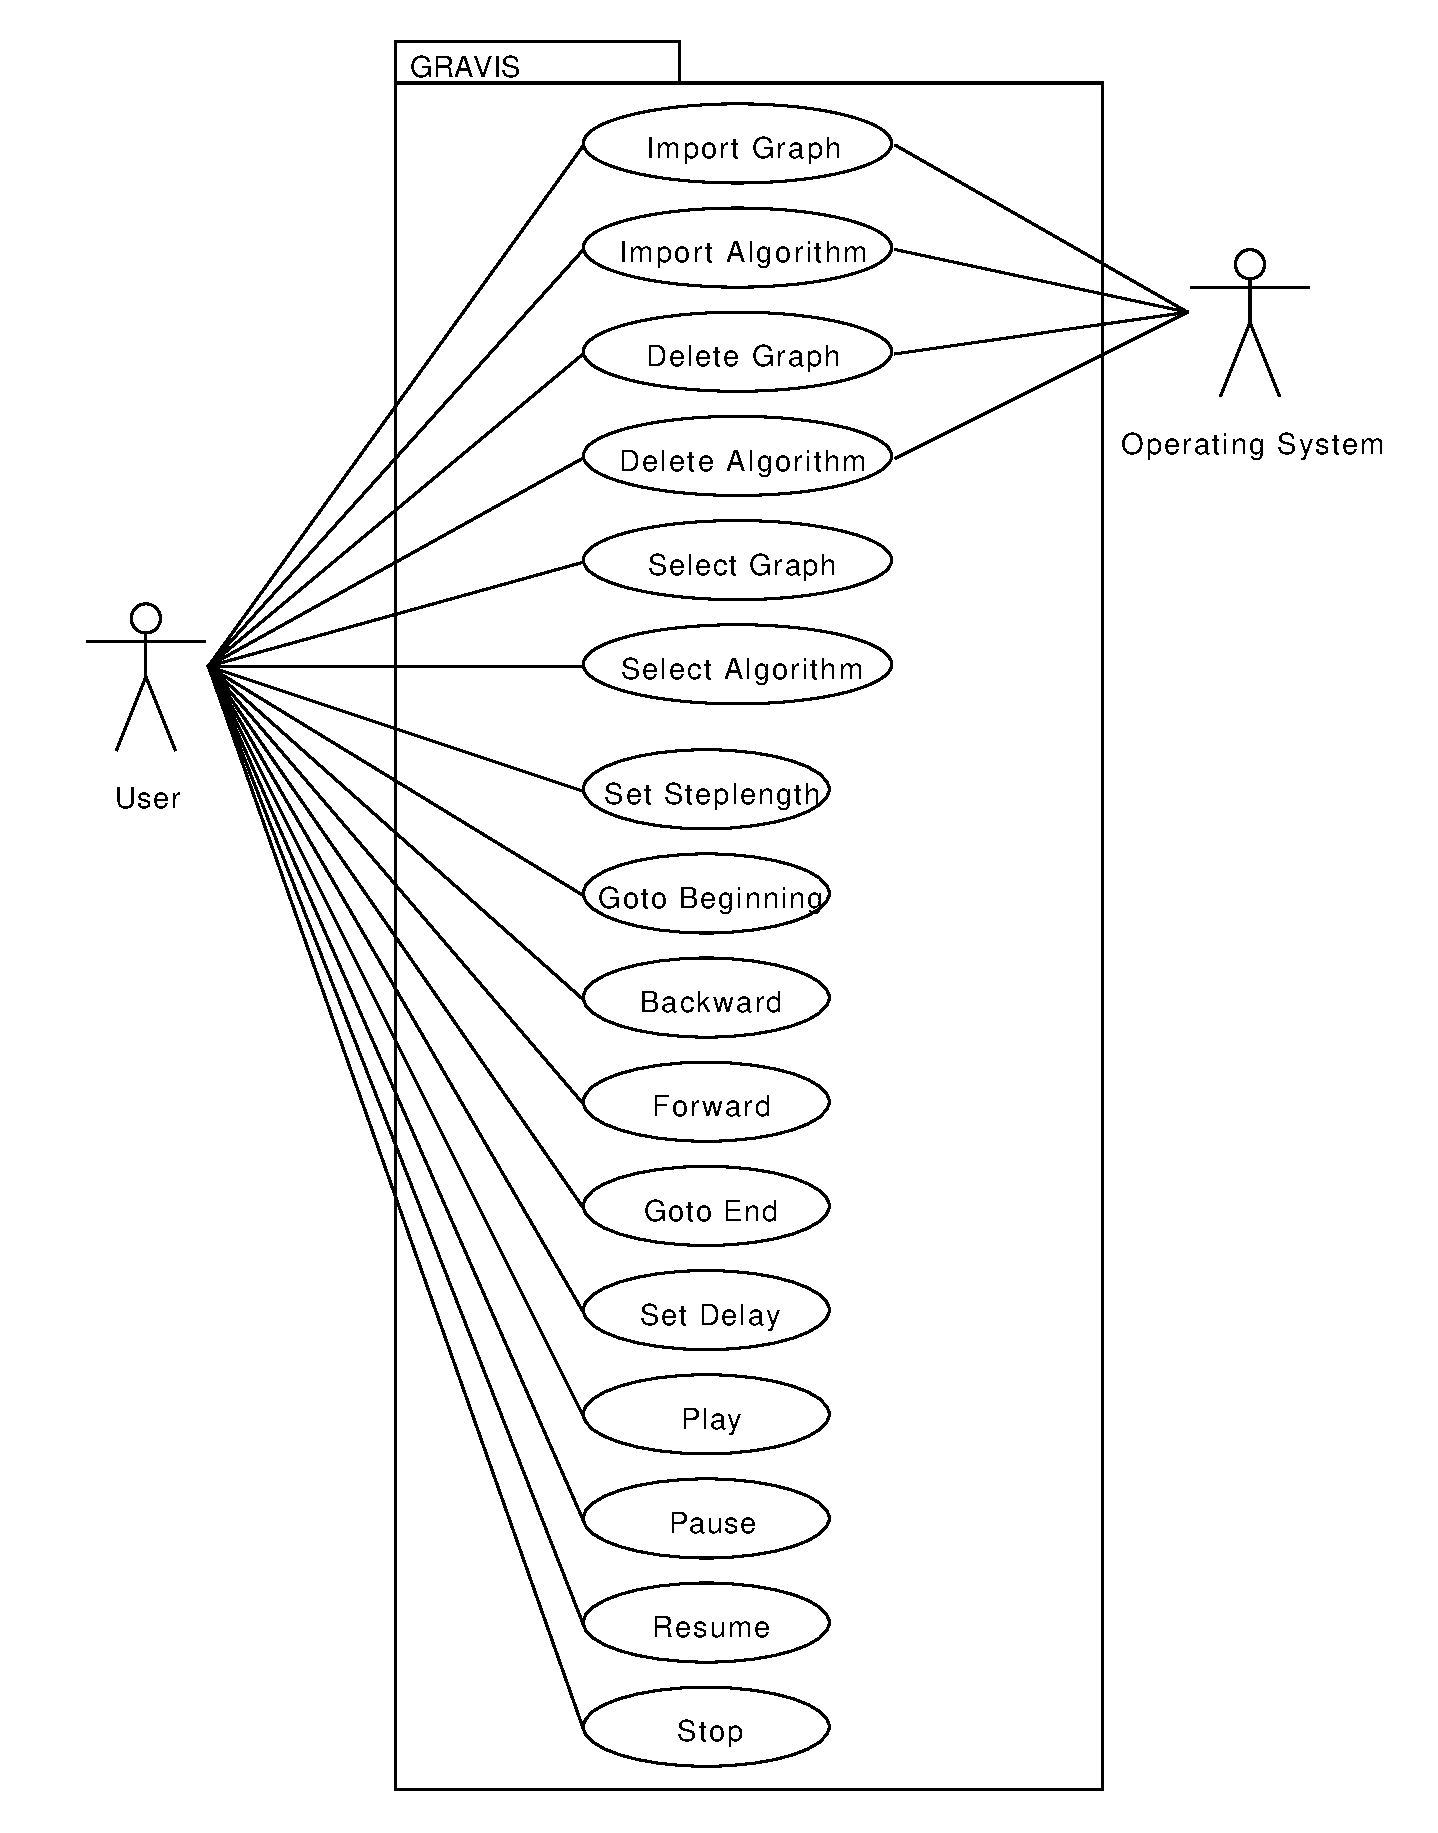
\includegraphics[scale=0.5]{diagrams/use-cases-diagram.pdf}
    \caption{Use Cases Diagram}
    \label{fig:use_cases_diagram}
\end{figure}
% 
\subsection{Use Cases in Brief Format}
\label{subsec:Use Cases in Brief Format}
% - All the use-cases of the application you discover, which have to be written in brief format;
\begin{description}
  \item[Import Graph:] Der User kann einen neuen Graphen importieren.

  (Ausgearbeitetes Format siehe Seite~\pageref{uc:Import Graph})

  \item[Import \Gls{Algorithm}:] Der User kann einen neuen Algorithmus importieren.

  (Ausgearbeitetes Format siehe Seite~\pageref{uc:Import Algorithm})

  \item[Delete Graph:] Der User kann einen importierten Graphen l\"oschen.

  (Ausgearbeitetes Format siehe Seite~\pageref{uc:Delete Graph})

  \item[Delete Algorithm:] Der User kann einen importierten Algorithmus l\"oschen.

  (Ausgearbeitetes Format siehe Seite~\pageref{uc:Delete Algorithm})

  \item[Select Graph:] Der User kann einen Graphen ausw\"ahlen.

  (Ausgearbeitetes Format siehe Seite~\pageref{uc:Select Graph})

  \item[Select Algorithm:] Der User kann einen Algorithmus ausw\"ahlen und damit eine Traversierung (\Gls{Traversal}) generieren.

  (Ausgearbeitetes Format siehe Seite~\pageref{uc:Select Algorithm})

  \item[Set \Gls{Steplength}:] Der User kann f\"ur die Visualisierung die Anzahl Traversierungsschritte (\Gls{Step}) pro Bild (\Gls{Image}) einstellen.

  \item[Forward:] Der User kann in der \Gls{Step-by-Step}-Visualisierung ein Bild vorw\"arts gehen.

  \item[Backward:] Der User kann in der Step-by-Step-Visualisierung ein Bild r\"uckw\"arts gehen.

  \item[Goto Beginning:] Der User kann in der Step-by-Step-Visualisierung an das Ende springen.

  \item[Goto End:] Der User kann in der Step-by-Step-Visualisierung an den Anfang springen.

  \item[Set \Gls{Delay}:] Der User kann f\"ur die animierte Visualisierung (\Gls{Animation}) das Zeitintervall zwischen zwei Bildern einstellen.

  \item[Play:] Der User kann die animierte Visualisierung starten.

  \item[Pause:] Der User kann die animierte Visualisierung pausieren.

  \item[Resume:] Der User kann die pausierte animierte Visualisierung wieder aktivieren.

  \item[Stop:] Der User kann die animierte Visualisierung anhalten.
\end{description}
% 
\subsection{Use Cases in Fully Dressed Format}
\label{subsec:Use Cases in Fully Dressed Format}
Die sechs UC \textit{Import Graph}, \textit{Import Algorithm}, \textit{Delete Graph}, \textit{Delete Algorithm}, \textit{Select Graph} und \textit{Select Algorithm} werden im ausgearbeiteten Format erl\"autert. F\"ur diese UC gilt:
\begin{itemize}
  \item Scope: System-wide
  \item Level: User-goal
  \item Primary Actor: User
\end{itemize}
\newpage
% 
\begin{usecase}{Import Graph}
    \preconditions{
	    \item Die Benutzerschnittstelle zur Befehlswahl ist aktiv.
	    \item Die Dateistruktur des Betriebssystems ist zug\"anglich.
	    \item Auf die zu importierende Datei sind mindestens Leserechte gesetzt.
    }
    \postconditions{
	    \item Der Parameter steht dem System zur weiteren Verarbeitung zur Verf\"ugung.
	    \item Der Parameter steht dem User in der Parameterliste zur Auswahl bereit.
            \item Der Default-Graph wurde ausgew\"ahlt.
    }
    \mainsuccess{
	    \item Der User w\"ahlt \"uber die Benutzerschnittstelle das Importieren eines Graphen (import).
	    \item Der User wird dazu aufgefordert, den Pfad und den Dateinamen einer Datei anzugeben (open) oder den Vorgang abzubrechen (abort).
	    \item Die angegebene Datei wird in die Dateistruktur des Systems kopiert (copy).
	    \item Die angegebene Datei wird durch das System auf Kompatibilit\"at gepr\"uft (load).
	    \item Der importierte Graph wird zur Graph-Parameterliste hinzugef\"ugt (add).
	    \item Der Default-Graph wird ausgew\"ahlt (select, siehe \textit{UC5 Select Graph} Seite~\pageref{uc:Select Graph}).
    }
\end{usecase}
\newpage 
% 
\begin{usecase}{Import Algorithm}
    \preconditions{
	    \item Die Benutzerschnittstelle zur Befehlswahl ist aktiv.
	    \item Die Dateistruktur des Betriebssystems ist zug\"anglich.
	    \item Auf die zu importierende Datei sind mindestens Leserechte gesetzt.
    }
    \postconditions{
	    \item Der Parameter steht dem System zur weiteren Verarbeitung zur Verf\"ugung.
	    \item Der Parameter steht dem User in der Parameterliste zur Auswahl bereit.
            \item Der Default-Graph wurde ausgew\"ahlt.
    }
    \mainsuccess{
	    \item Der User w\"ahlt \"uber die Benutzerschnittstelle das Importieren eines Algorithm (import).
	    \item Der User wird dazu aufgefordert, den Pfad und den Dateinamen einer Datei anzugeben (open) oder den Vorgang abzubrechen (abort).
	    \item Die angegebene Datei wird in die Dateistruktur des Systems kopiert (copy).
	    \item Die angegebene Datei wird durch das System auf Kompatibilit\"at gepr\"uft (load).
	    \item Der importierte Algorithmus wird zur Algorithmus-Parameterliste hinzugef\"ugt (add).
	    \item Der Default-Algorithm wird ausgew\"ahlt (select, siehe \textit{UC6 Select Algorithm} Seite~\pageref{uc:Select Algorithm}).
    }
\end{usecase}
\newpage 
% 
\begin{usecase}{Delete Graph}
    \preconditions{
	    \item Die Benutzerschnittstelle zur Befehlswahl ist aktiv.
	    \item Die Dateistruktur des Betriebssystems ist zug\"anglich.
	    \item Auf die zu l\"oschende Datei sind Schreibrechte gesetzt.
    }
    \postconditions{
	    \item Die Datei wurde aus dem System gel\"oscht.
	    \item Die Graph-Parameterliste wurde aktualisiert.
            \item Der Default-Graph wurde ausgew\"ahlt.
    }
    \mainsuccess{
	    \item Der User w\"ahlt ahlt \"uber die Benutzerschnittstelle das L\"oschen eines Graphen (delete).
	    \item Der User wird dazu aufgefordert, den Pfad und den Dateinamen der Datei anzugeben (open) oder den Vorgang abzubrechen (abort).
	    \item Der zu l\"oschende Graph wird aus der Graph-Parameterliste entfernt (remove).
	    \item Die angegebene Datei wird aus der Dateistruktur des Systems gel\"oscht (delete).
	    \item Der Default-Graph wird ausgew\"ahlt (select, siehe \textit{UC5 Select Graph} Seite~\pageref{uc:Select Graph}).
    }
\end{usecase}
\newpage 
% 
\begin{usecase}{Delete Algorithm}
    \preconditions{
	    \item Die Benutzerschnittstelle zur Befehlswahl ist aktiv.
	    \item Die Dateistruktur des Betriebssystems ist zug\"anglich.
	    \item Auf die zu l\"oschende Datei sind Schreibrechte gesetzt.
    }
    \postconditions{
	    \item Die Datei wurde aus dem System gel\"oscht.
	    \item Die Algorithm-Parameterliste wurde aktualisiert.
            \item Der Default-Graph wurde ausgew\"ahlt.
    }
    \mainsuccess{
	    \item Der User w\"ahlt ahlt \"uber die Benutzerschnittstelle das L\"oschen eines Algorithm (delete).
	    \item Der User wird dazu aufgefordert, den Pfad und den Dateinamen der Datei anzugeben (open) oder den Vorgang abzubrechen (abort).
	    \item Der zu l\"oschende Algorithm wird aus der Algorithm-Parameterliste entfernt (remove).
	    \item Die angegebene Datei wird aus der Dateistruktur des Systems gel\"oscht (delete).
	    \item Der Default-Algorithm wird ausgew\"ahlt (select, siehe \textit{UC6 Select Algorithm} Seite~\pageref{uc:Select Algorithm}).
    }
\end{usecase}
\newpage 
% 
\begin{usecase}{Select Graph}
    \precondition{
	    Die Benutzerschnittstelle zur Wahl eines Graphen ist aktiv.
    }
    \postconditions{
	    \item Der Graph wurde als ausgew\"ahlt markiert.
	    \item Der gew\"ahlte Graph steht als geladene Instanz zur weiteren Verarbeitung zur Verf\"ugung.
	    \item Der gew\"ahlte Graph ist visualisiert.
	    \item Die auf den Graphen anwendbaren Algorithmen wurden aktiv gesetzt.
	    \item Die Parameterlisten der Benutzerschnittstellen wurden aktualisiert.
    }
    \mainsuccess{
	    \item Der vormalige Graph wird im System entladen (clear).
	    \item Der gew\"ahlte Graph wird ins System geladen (load).
	    \item In der Parameterliste wird der gew\"ahlte Graph als aktuell gesetzt (set selected).
	    \item Die auf den Graphen anwendbaren Algorithm werden aktiv gesetzt (enable).
	    \item Die Parameterlisten der Benutzerschnittstellen werden aktualisiert.
	    \item Der aktuelle Graph wird im Visualizer dargestellt.
    }
\end{usecase}
\newpage 
% 
\begin{usecase}{Select Algorithm}
    \preconditions{
	    \item Die Benutzerschnittstelle zur Wahl eines Algorithm ist aktiv.
    }
    \postconditions{
	    \item Der Algorithm wurde als ausgew\"ahlt markiert (\textit{selected}).
	    \item Der gew\"ahlte Algorithm wurde als Instanz geladen.
	    \item Die Parameterliste der Benutzerschnittstelle wurde aktualisiert.
            \item Der gew\"ahlte Algorithm hat eine Traversal generiert.
	    \item Das System ist zur Visualisierung der Traversal bereit.
    }
    \mainsuccess{
	    \item In der Parameterliste wird der gew\"ahlte Algorithm als ausgew\"ahlt markiert (\textit{selected}).
	    \item Der gew\"ahlte Algorithm wird ins System geladen.
	    \item Die Parameterliste der Benutzerschnittstelle wurde aktualisiert.
	    \item Der gew\"ahlte Algorithm brechnet die Traversal.
	    \item Der User erh\"alt eine Mitteilung, dass die Berechnung der Traversal abgeschlossen ist.
	    \item Der User quittiert die Mitteilung.
	    \item Die Abspielkonsole zur Steuerung der Visualisierung wird aktiviert.
    }
\end{usecase} 			% Use Cases
\section{Supplementary Specification}
\label{sec:Supplementary Specification}
\begin{description}
  \item[Platform:] Das System soll auf verschiedenen Betriebssystemen lauff\"ahig sein, im minimum auf GNU/Linux, Mac OS und Microsoft Windows.
  \item[I18n:] Das System soll in den drei Sprachen Deutsch, Franz\"osisch und Englisch bedienbar sein.
\end{description}
% 
\section{Glossary}
\label{sec:Glossary}
% Key domain terminology and data dictionary.
\begin{description}
  \item[Algorithm] -- Algorithmus: Anleitung, wie ein Graph durchschritten werden soll.
  \item[Traversal] -- Traversierung: Durchf\"uhrung eines Algorithmus und Sammlung der Traversierungsschritte als Resultat. Der Graph erf\"ahrt bei jedem Traversierungsschritt eine \`Anderung seines Zustandes.
  \item[Step] -- Einzelner Schritt der Traversierung.
  \item[Image] -- Bild: Darstellung eines Zustandes eines Graphen.
  \item[Step-by-Step] -- Visualisierung, bei der ein Bild-Wechsel durch eine Benutzerinteraktion erfolgt.
  \item[Steplength] -- Anzahl Schritte (Steps) pro Bild-Wechsel.
  \item[Animation] -- Visualisierung, bei der der Bild-Wechsel wiederholt automatisch, also ohne Benutzerinteraktion erfolgt.
  \item[Delay] -- F\"ur die Animation: Verstreichende Zeit zwischen einem Bild-Wechsel.
\end{description}
% 
% \section{Domain Rules}
% \label{sec:Domain Rules}
% Key business and domain rules. 			% Supplementary Specification, Domain Rules
% Design
\chapter{Design}
% 
\section{Domain Model}
\label{sec:Domain Model}
% 
\subsection{Domain Model Diagram}
\label{subsec:Domain Model Diagram}
\begin{figure}[H]
    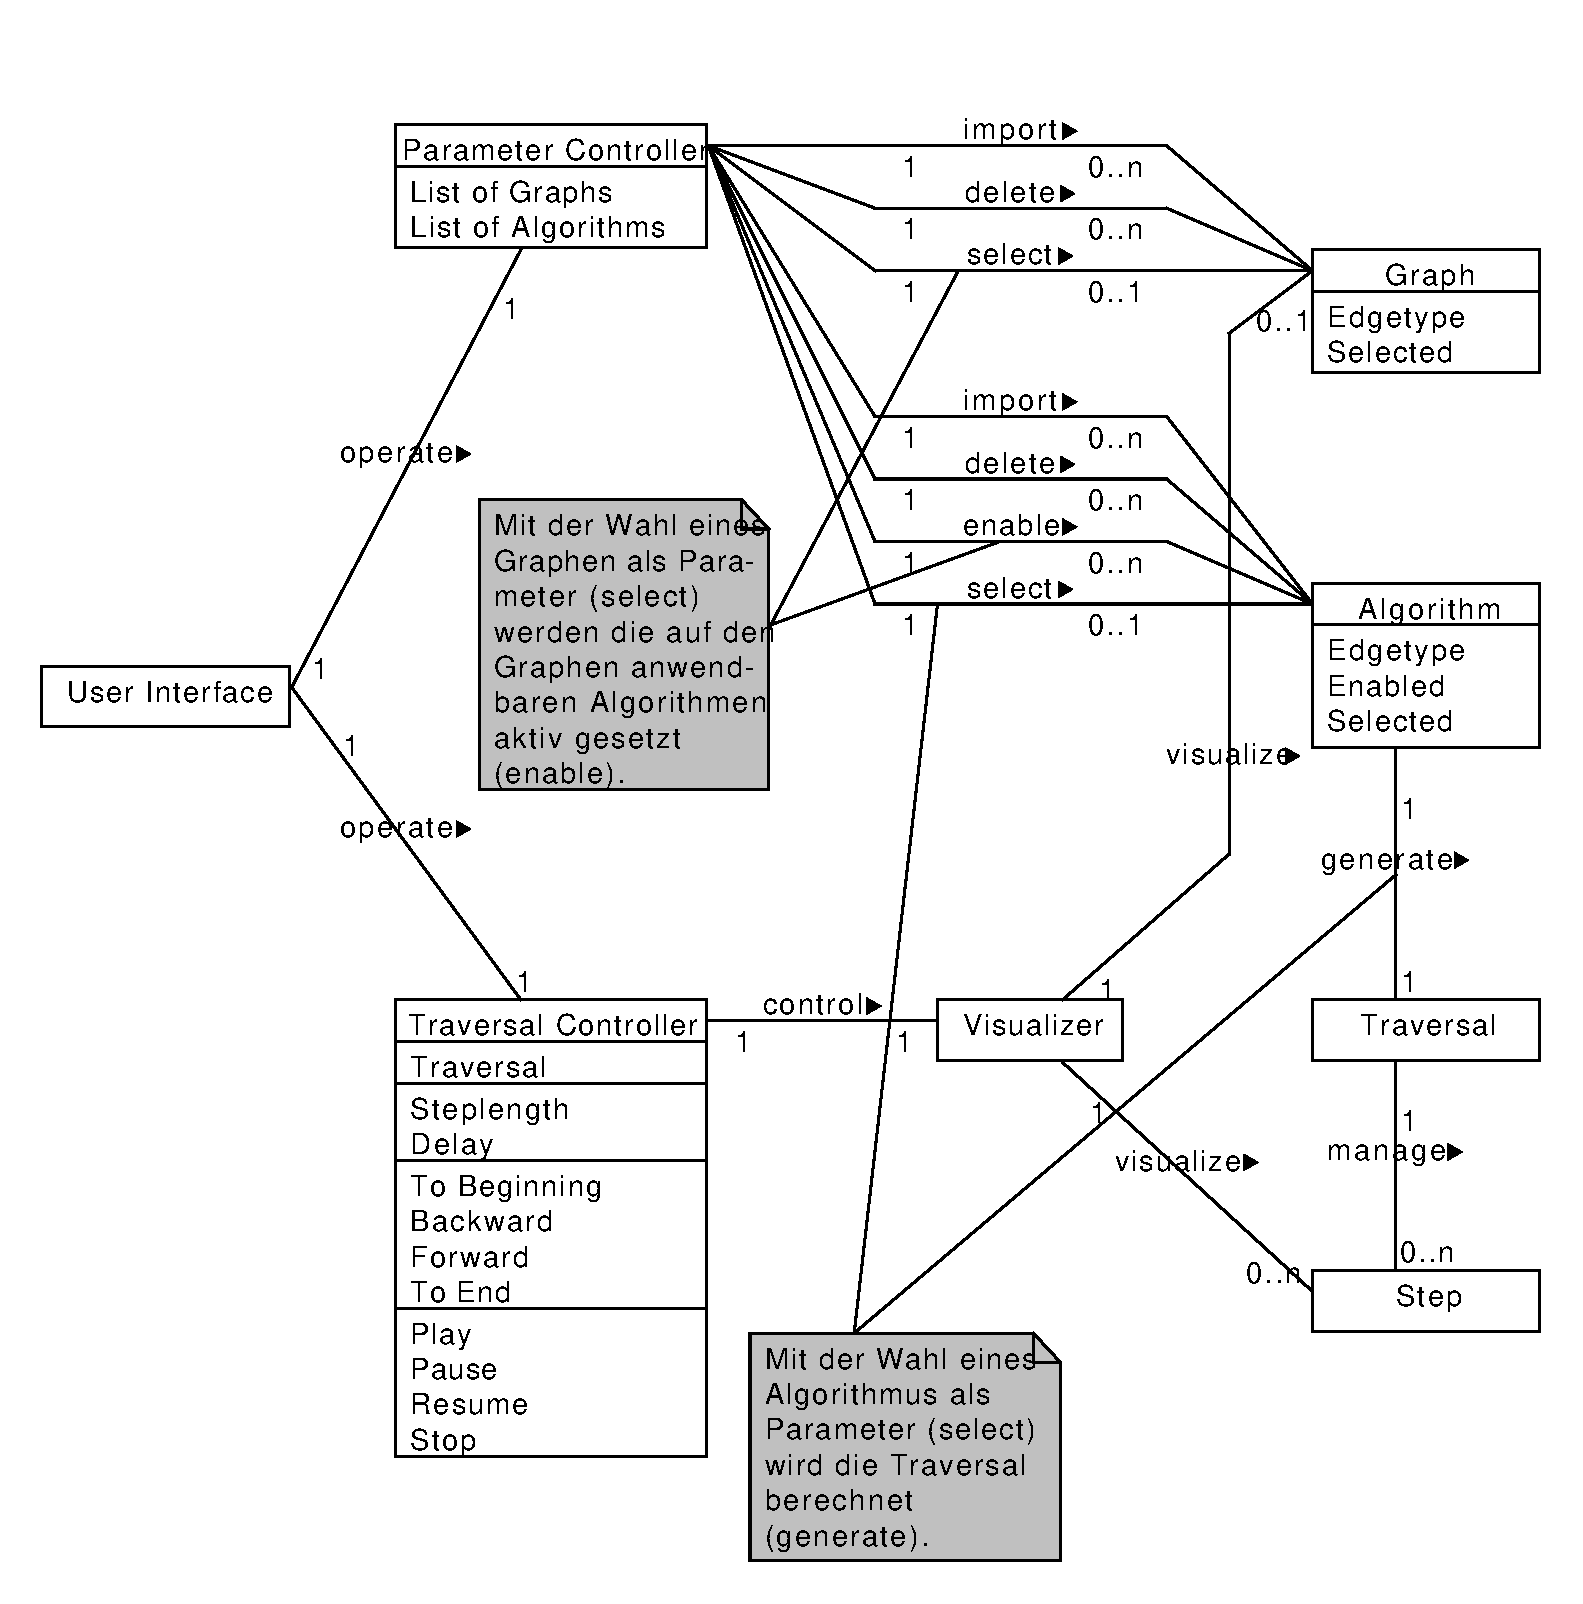
\includegraphics[totalheight=0.6\textheight]{diagrams/domain-model-diagram.pdf}
    \caption{Domain Model Diagram}
    \label{fig:domain_model_diagram}
\end{figure}
% 
\subsection{Domain Model Description}
\label{subsec:Domain Model Description}
Es folgt eine Beschreibung der Konzeptklassen (conceptual classes) mit Assoziationen, wie im Domain Model Diagram gezeigt. Multiplizit\"aten und Attribute werden in Klammern angegeben.
% 
\subsubsection{User Interface}
\label{subsubsec:User Interface}
\begin{itemize}
  \item \"Uber ein User Interface (1) kann ein User einen Parameter Controller (1) bedienen (\textit{operate}).
  \item \"Uber ein User Interface (1) kann ein User einen Traversal Controller (1) bedienen (\textit{operate}).
\end{itemize}
% 
\subsubsection{Parameter Controller}
\label{subsubsec:Parameter Controller}
\begin{itemize}
  \item Ein Parameter Controller verwaltet die zur Traversal ben\"otigten Parameter Graph (\textit{List of Graphs}) und Algorithm (\textit{List of Algorithms}).
  \item Der Parameter Controller h\"alt eine gegebene Anzahl von Graphen als Vorlagen bereit.
  \item Per Parameter Controller (1) kann ein User einen oder mehrere Graphen (0..n) des Formates *.graphml importieren (\textit{import}). Die importierten Graphen werden der Liste mit Graphen (\textit{List of Graphs}) hinzugef\"ugt.
  \item Per Parameter Controller (1) kann ein User vormals importierte Graphn (0..n) wieder l\"oschen (\textit{delete}). Diese werden aus der Liste mit Graphen (\textit{List of Graphs}) wieder entfernt.
  \item Per Parameter Controller (1) kann ein User einen Graphen (0..1) als Parameter ausw\"ahlen (\textit{select}).
  \item Mit der Wahl eines Graphen (1) als Parameter werden die auf den Graphen anwendbaren Algorithmen (0..n) aktiv gesetzt (\textit{enable}).
  \item Ein Parameter Controller h\"alt eine gegebene Anzahl Algorithmen als Vorlagen bereit.
  \item Per Parameter Controller (1) kann ein User einen oder mehrere Algorithmen (0..n) importieren (\textit{import}), sofern diese ein gefordertes Interface implementieren. Die importierten Algorithmen werden der Liste mit Algorithmen (\textit{List of Algorithms}) hinzugef\"ugt.
  \item Per Parameter Controller (1) kann ein User vormals importierte Algorithmen (0..n) wieder l\"oschen (\textit{delete}). Diese werden aus der Liste mit Algorithmen (\textit{List of Algorithms}) wieder entfernt.
  \item Per Parameter Controller (1) kann ein User einen aktivierten (\textit{Enabled}) Algorithmus (0..1) als Parameter ausw\"ahlen (\textit{select}).
\end{itemize}
% 
\subsubsection{Graph}
\label{subsubsec:Graph}
\begin{itemize}
  \item Ein Graph hat ungerichtete oder gerichtete Kanten (\textit{Edgetype}).
  \item Ein Graph kann ausgew\"ahlt werden (\textit{Selected}).
\end{itemize}
% 
\subsubsection{Algorithm}
\label{subsubsec:Algorithm}
\begin{itemize}
  \item Ein Algorithm kann Graphen mit ungerichteten oder gerichteten Kanten (\textit{Edgetype}) verarbeiten.
  \item Ein Algorithm (1) generiert eine Traversal (1) (\textit{generate}).
  \item Ein Algorithm kann aktiviert werden (\textit{Enabled}).
  \item Ein aktivierter Algorithm (\textit{Enabled}) kann ausgew\"ahlt werden (\textit{Selected}).
  \item Mit der Wahl eines Algorithm (1) als Parameter (\textit{Selected}) wird eine Traversal (1) erstellt (\textit{generate}).
\end{itemize}
% 
\subsubsection{Traversal}
\label{subsubsec:Traversal}
\begin{itemize}
  \item Die Traversierung ist ein visualisierbares Objekt.
  \item Eine Traversal (1) kann einen oder mehrere Steps (0..n) verwalten (\textit{manage}).
\end{itemize}

\subsubsection{Step}
\label{subsubsec:Step}
\begin{itemize}
  \item Ein Step ist ein Schritt der Traversierung.
\end{itemize}

\subsubsection{Traversal Controller}
\label{subsubsec:Traversal Controller}
\begin{itemize}
  \item Ein Traversal Controller (1) steuert einen Visualizer (1) (\textit{control}).
  \item Der Traversal Controller h\"alt eine Traversierung (\textit{Traversal}).
  \item Per Traversal Controller kann ein User die Anzahl Schritte pro Bild (\textit{Steplength}) einstellen.
  \item Per Traversal Controller kann ein User die Zeit zwischen zwei Bildern (\textit{Delay}) einstellen.
  \item Per Traversal Controller kann ein User Step-by-Step-Elemente (\textit{Forward, Backward, To Beginning, To End}) bedienen.
  \item Per Traversal Controller kann ein User Animations-Elemente (\textit{Play, Pause, Resume, Stop}) bedienen.
\end{itemize}

\subsubsection{Visualizer}
\label{subsubsec:Visualizer}
\begin{itemize}
  \item Ein Visualizer (1) kann einen Graphen (0..1) visualisieren (\textit{visualize}).
  \item Ein Visualizer (1) kann einen oder mehrere Steps (0..n) visualisieren (\textit{visualize}).
\end{itemize} 			% Domain Model, Design Model
\section{Design Model}
\label{sec:design-model}
This design model affects previous artifacts with changes as follows:
\begin{itemize}
  \item The \textbf{Use Cases} got renamed to \textit{Register}, \textit{Subscribe}, \textit{Consult Articles}, \textit{Upload Articles} and \textit{Upload Issue}. 
  \item One more \textbf{Use Case} named \textit{Fetch Articles} has been added in brief format.
  \item The \textbf{Use Cases} in fully dressed format (\textit{Register}, \textit{Subscribe}, \textit{Upload Articles} and \textit{Fetch Articles}) got rewritten.
  \item The \textbf{Use Case Diagram} got updated.
  \item The \textbf{Domain Model Diagram} and the \textbf{Domain Model Description} got updated, some multiplicities have changed (e.g. for \textit{Article}).
\end{itemize}

As mentioned earlier the ENL system is a typical client-server application. We develop the server side only, therefore we focus on the user interaction related Use Cases \textit{Register}, \textit{Subscribe}, \textit{Consult Articles}, \textit{Upload Article}, \textit{Fetch Articles} and \textit{Upload Issue}. For each of them, this documentation serves with
\begin{itemize}
  \item a \textbf{System Sequence Diagram (SSD)} illustrating how certain tasks are done between users and the system, 
  \item a \textbf{Sequence Diagram (SD)} illustrating how objects collaborate together in the server and what the responsibilities of the classes are, 
  \item and a \textbf{Design Class Diagram (DCD)} illustrating the static aspects of the server side of the ENL system with respect of the functionality.
\end{itemize}

Every system event will be associated to a single system operation of a controller. Moreover, a controller implements exclusively system operations (and maybe some privates methods). Generally, classes of our design do not call methods of any controllers.
\newpage

\subsection{Login}
\label{subsec:login}
\begin{figure}[H]
    \includegraphics[width=\textwidth]{diagrams/sd/sd-login.png}
    \caption{Login, Sequence Diagram}
    \label{fig:login-sd}
\end{figure}
\newpage

\subsection{Register}
\label{subsec:register}
\begin{figure}[H]
    \includegraphics[width=\textwidth]{diagrams/ssd/ssd-register.pdf}
    \caption{Register, System Sequence Diagram}
    \label{fig:register-ssd}
\end{figure}
% \newpage
\begin{figure}[H]
    \includegraphics[width=\textwidth]{diagrams/sd/sd-register.png}
    \caption{Register, Sequence Diagram}
    \label{fig:register-sd}
\end{figure}
\newpage
\begin{figure}[H]
    \includegraphics[width=\textwidth]{diagrams/dcd/dcd-register.png}
    \caption{Register, Design Class Diagram}
    \label{fig:register-dcd}
\end{figure}
\newpage

\subsection{Subscribe}
\label{subsec:subscribe}
\begin{figure}[H]
    \includegraphics[width=\textwidth]{diagrams/ssd/ssd-subscribe.pdf}
    \caption{Subscribe, System Sequence Diagram}
    \label{fig:subscribe-ssd}
\end{figure}
\newpage
% \begin{figure}[H]
%     \includegraphics[width=\textwidth]{diagrams/sd/sd-subscribe.pdf}
%     \caption{Subscribe, Sequence Diagram}
%     \label{fig:subscribe-sd}
% \end{figure}
% \newpage
% \begin{figure}[H]
%     \includegraphics[width=\textwidth]{diagrams/dcd/dcd-subscribe.pdf}
%     \caption{Subscribe, Design Class Diagram}
%     \label{fig:subscribe-dcd}
% \end{figure}
% \newpage

\subsection{Consult Articles}
\label{subsec:consult-articles}
\begin{figure}[H]
    \includegraphics[width=\textwidth]{diagrams/ssd/ssd-consult-articles.pdf}
    \caption{Consult-Articles, System Sequence Diagram}
    \label{fig:consult-articles-ssd}
\end{figure}
\newpage
% \begin{figure}[H]
%     \includegraphics[width=\textwidth]{diagrams/sd/sd-consult-articles.pdf}
%     \caption{Consult-Articles, Sequence Diagram}
%     \label{fig:consult-articles-sd}
% \end{figure}
% \newpage
% \begin{figure}[H]
%     \includegraphics[width=\textwidth]{diagrams/dcd/dcd-consult-articles.pdf}
%     \caption{Consult-Articles, Design Class Diagram}
%     \label{fig:consult-articles-dcd}
% \end{figure}
% \newpage

\subsection{Upload Article}
\label{subsec:upload-article}
\begin{figure}[H]
    \includegraphics[width=\textwidth]{diagrams/ssd/ssd-upload-article.pdf}
    \caption{Upload-Article, System Sequence Diagram}
    \label{fig:upload-article-ssd}
\end{figure}
\newpage
% \begin{figure}[H]
%     \includegraphics[width=\textwidth]{diagrams/sd/sd-upload-article.pdf}
%     \caption{Upload-Article, Sequence Diagram}
%     \label{fig:upload-article-sd}
% \end{figure}
% \newpage
% \begin{figure}[H]
%     \includegraphics[width=\textwidth]{diagrams/dcd/dcd-upload-article.pdf}
%     \caption{Upload-Article, Design Class Diagram}
%     \label{fig:upload-article-dcd}
% \end{figure}
% \newpage

\subsection{Fetch Articles}
\label{subsec:fetch-articles}
\begin{figure}[H]
    \includegraphics[width=\textwidth]{diagrams/ssd/ssd-fetch-articles.pdf}
    \caption{Fetch-Articles, System Sequence Diagram}
    \label{fig:fetch-articles-ssd}
\end{figure}
\newpage
% \begin{figure}[H]
%     \includegraphics[width=\textwidth]{diagrams/sd/sd-fetch-articles.pdf}
%     \caption{Fetch-Articles, Sequence Diagram}
%     \label{fig:fetch-articles-sd}
% \end{figure}
% \newpage
% \begin{figure}[H]
%     \includegraphics[width=\textwidth]{diagrams/dcd/dcd-fetch-articles.pdf}
%     \caption{Fetch-Articles, Design Class Diagram}
%     \label{fig:fetch-articles-dcd}
% \end{figure}
% \newpage

\subsection{Upload Issue}
\label{subsec:upload-issue}
\begin{figure}[H]
    \includegraphics[width=\textwidth]{diagrams/ssd/ssd-upload-issue.pdf}
    \caption{Upload-Issue, System Sequence Diagram}
    \label{fig:upload-issue-ssd}
\end{figure}
\newpage
% \begin{figure}[H]
%     \includegraphics[width=\textwidth]{diagrams/sd/sd-upload-issue.pdf}
%     \caption{Upload-Issue, Sequence Diagram}
%     \label{fig:upload-issue-sd}
% \end{figure}
% \newpage
% \begin{figure}[H]
%     \includegraphics[width=\textwidth]{diagrams/dcd/dcd-upload-issue.pdf}
%     \caption{Upload-Issue, Design Class Diagram}
%     \label{fig:upload-issue-dcd}
% \end{figure}
% \newpage 			% Design Model: diagrams
\section{Software Architecture Document}
\label{sec:Software Architecture Document}
% 
% \subsection{Architektonische Repr\"asentation}
% 
% 
% \subsection{Architektonische Faktoren}
% 
% 
\subsection{Architektonische Entscheidungen}
% 
\subsubsection{Matrixmultiplikation}
Brainstorming zu Beginn des Projektes: Kybernetisches System mit
\begin{itemize}
  \item Operand: Graph als Adjazenz-Matrix
  \item Operator: e.g. Dijkstra-Algorithmus (als Matrix)
  \item Transition: Ein Schritt der Traversierung
  \item Transformierte: Graph im neuen Zustand
\end{itemize}
Berechnung der Traversierung per Matrixmultiplikation:
\begin{itemize}
  \item Definition der Operatoren (Algorithmen) allgemein g\"ultig als Matrizen
  \item Anwenden der Operatoren (Algorithmen) auf Operanden (Graphen) als Matrixmultiplikation
  \item Resultat: Liste von (bijektiven, also eineindeutigen) Transformationen ('Steps') als Matrizenmechanik
\end{itemize}
% 
\subsubsection{Entscheidungen}
% 
\begin{itemize}
  \item Themenkreis Matrizen: Entscheid, dass keine Matrizen-Multiplikation. Implementation mit Bezug auf \textit{Algorithm Design} von M. Goodrich und R. Tamassia~\cite{goodrichtamassia:2002}.
  \item Zu Projektbeginn wurde relativ bald eine Drei-Schichten-Architektur entworfen.
  \item In der Woche 45 wurde entschieden, das Projekt als Maven-Projekt zu halten. Der Entscheid wurde vorallem getroffen, da Properties zentral verwaltet und Tests sauber vom restlichen Sourcecode getrennt gehalten werden k\"onnen.
\end{itemize}
% 
% \subsection{Logical View}
% 
% \subsubsection{Beschreibung und Motivation}
% 
% \subsection{Deployment View}
% 
% \subsubsection{Beschreibung und Motivation}
% 
\subsection{Process View}
% 
\begin{figure}[H]
    \centering
    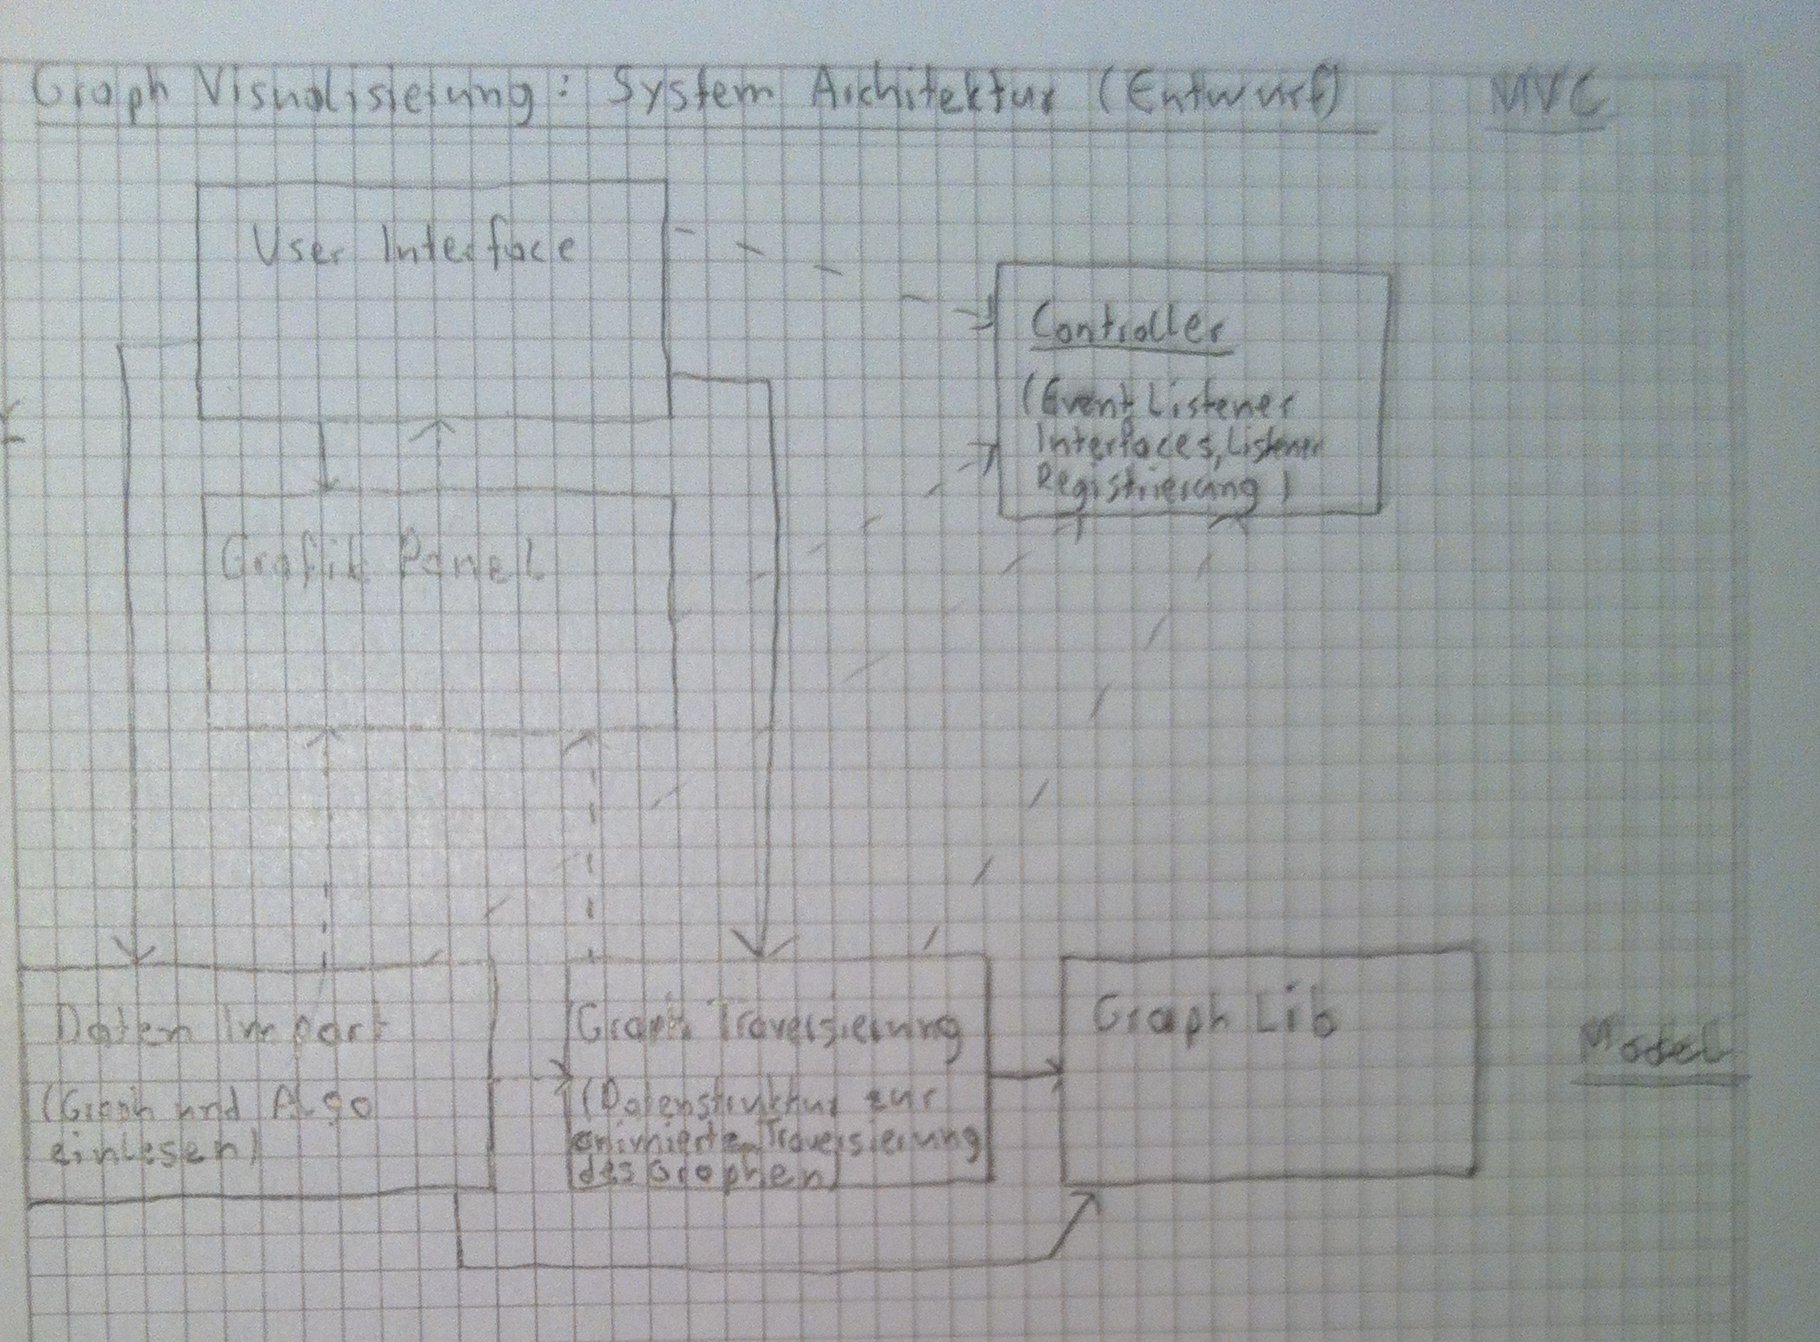
\includegraphics[
% 		    width=\textwidth,
% 		    height=\textheight,
% 		    angle=90,
		    scale=0.1,
		    keepaspectratio=true
    ]{diagrams/Draft_System_Architecture_PK_V1_cropped.jpeg}
    \caption{Gui, MVC: Conceptual Class Diagram}
    \label{fig:gui-mvc-ccd}
\end{figure}
% 
\subsection{Use-Case View}
Folgende Use Cases wurden implementiert:
\begin{itemize}
  \item Daten:
  \begin{itemize}
    \item Neuen Graphen oder Algorithmus importieren
    \item Importierter Graph oder Algorithmus l\"oschen
  \end{itemize}
  \item Traversierung:
  \begin{itemize}
    \item Graph ausw\"ahlen
    \item Algorithmus ausw\"ahlen
%     \item evt. Start- resp. Endknoten ausw\"ahlen
  \end{itemize}
  \item Visualisierung:
  \begin{itemize}
      \item Einstellen Steplength: Anzahl Traversierungs-Schritte pro Bild
      \item Einstellen Delay: Zeitintervall zwischen zwei Bildern (in Sekunden)      
      \item Visualisierung, Step-by-Step: Ein Bild vor, ein Bild zur\"uck, an das Ende oder den an den Anfang springen
      \item Visualisierung, Animation: Starten, Anhalten, Stoppen
  \end{itemize}
\end{itemize}
% 
\begin{figure}[H]
    \centering
    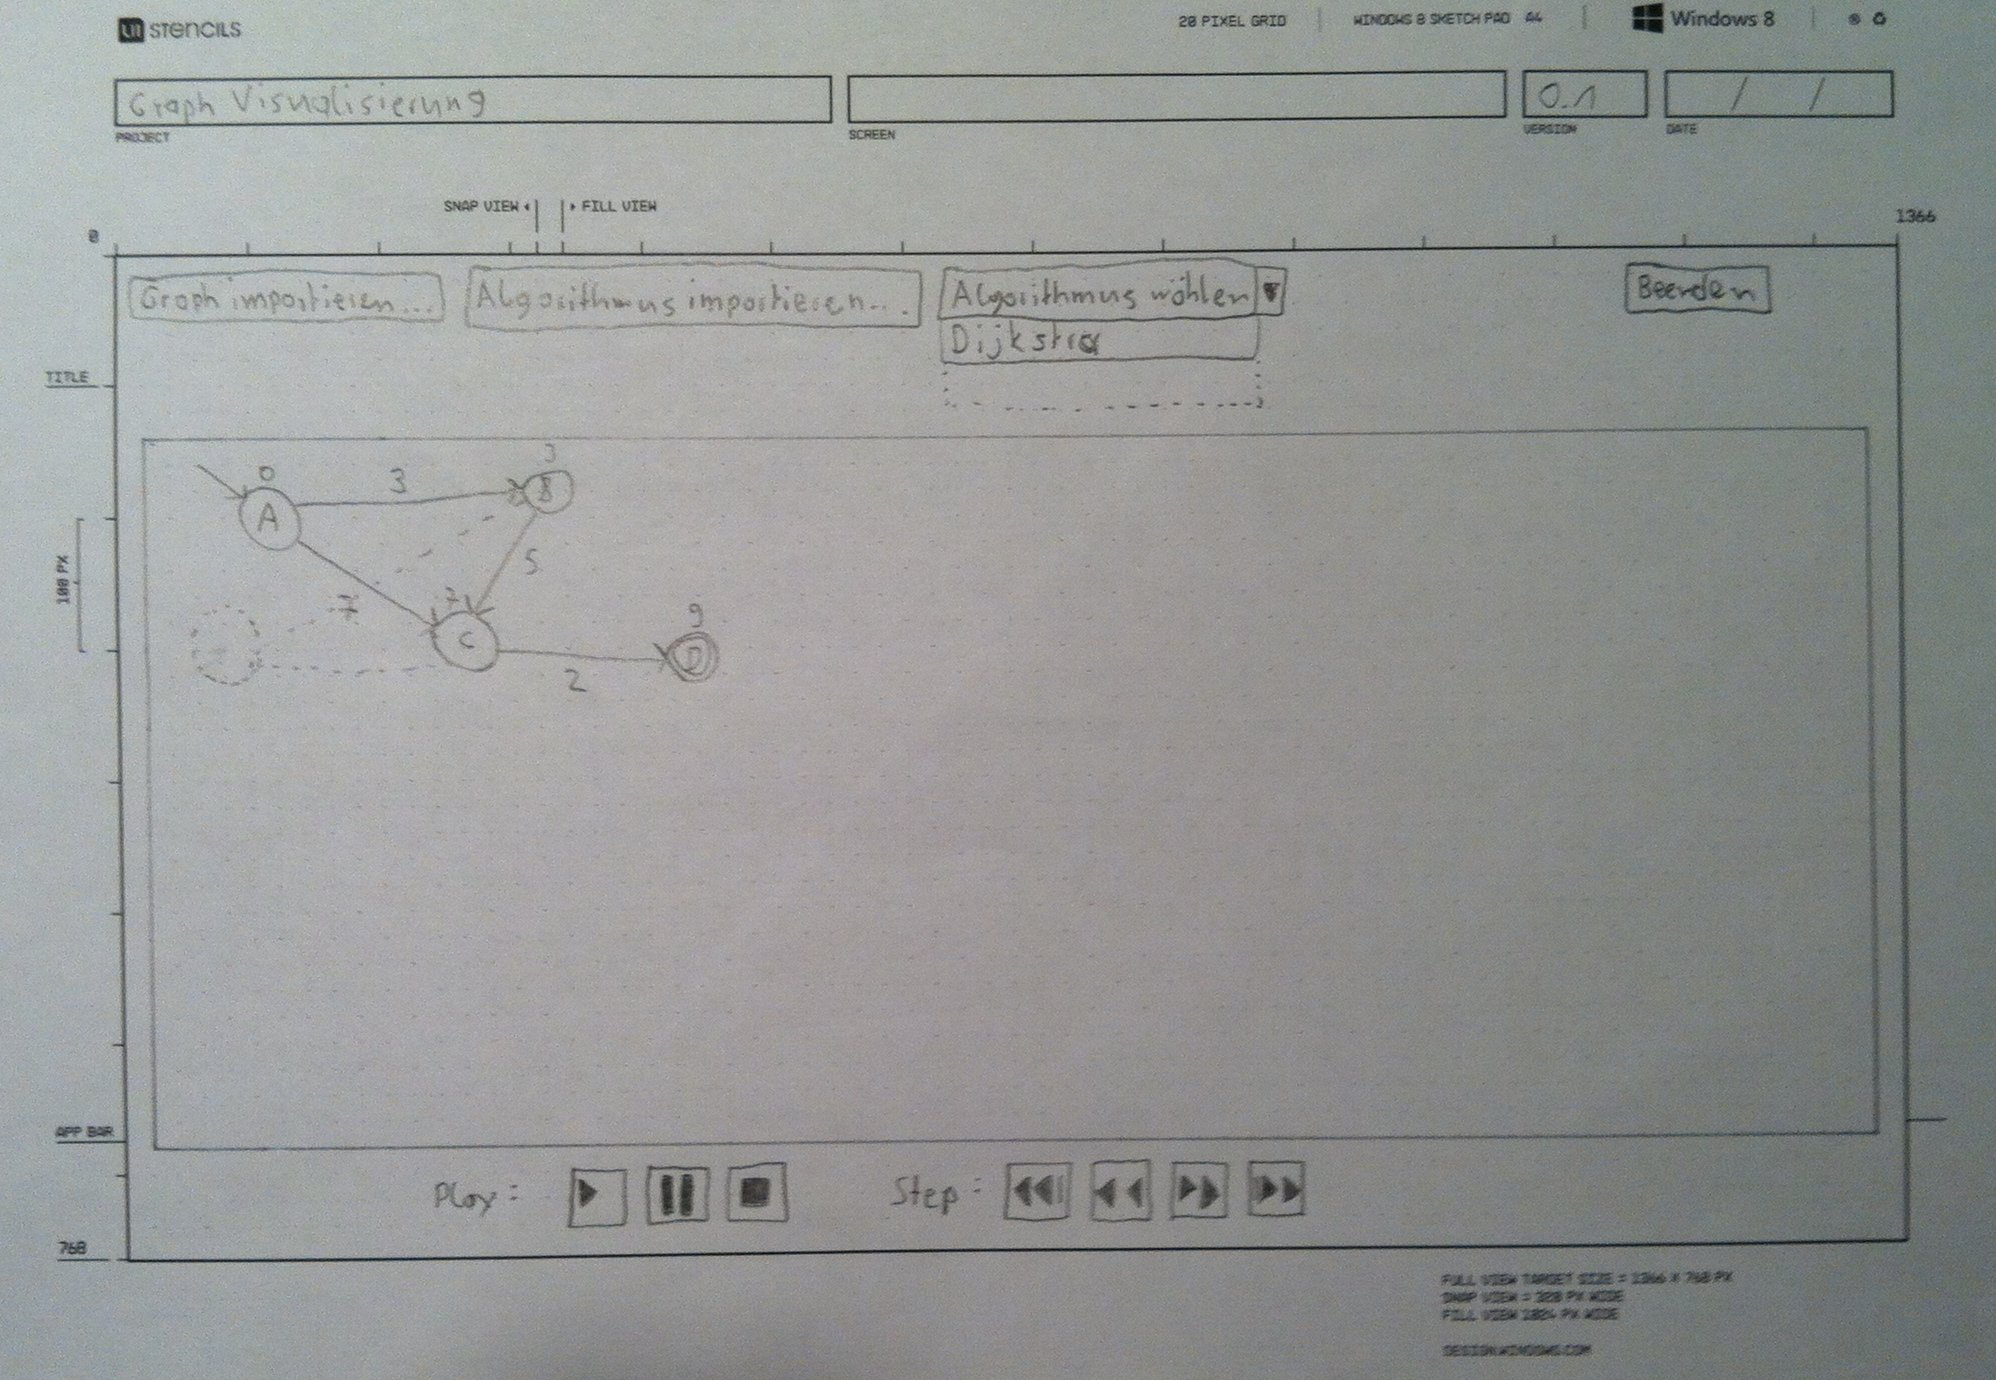
\includegraphics[
% 		    width=\textwidth,
% 		    height=\textheight,
% 		    angle=90,
		    scale=0.1,
		    keepaspectratio=true
    ]{diagrams/Screen_Sketch_PK_V1_cropped.jpeg}
    \caption{Gui, View: Screen Sketch}
    \label{fig:gui-view-screen-sketch}
\end{figure}
% 
\begin{figure}[H]
    \centering
    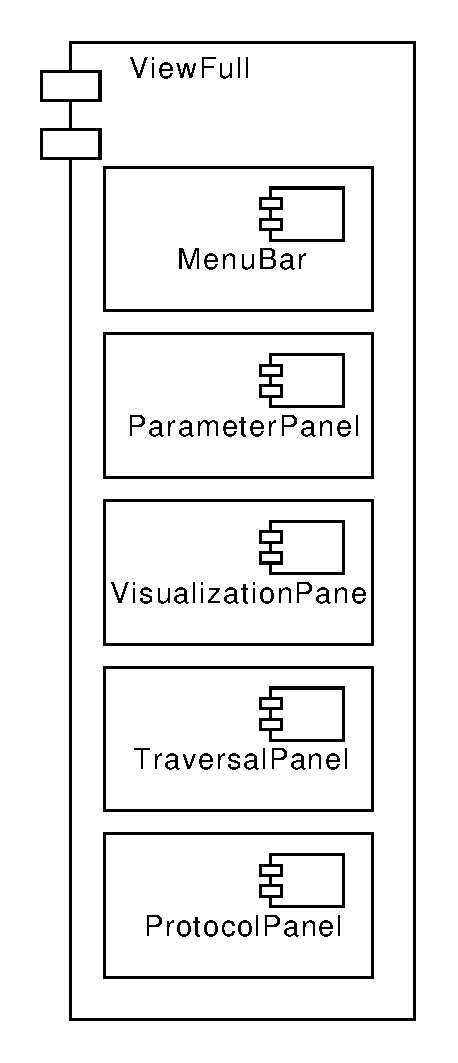
\includegraphics[scale=0.5]{diagrams/designmodel/cd-view-full.pdf}
    \caption{Gui, View: Component Diagram}
    \label{fig:gui-view-cd}
\end{figure} 			% Software Architecture Document
% Project Management
\chapter{Project Management}
% 
\section{Time Management}
\label{sec:Time Management}
Das Modul BTI-7301 Projekt 1 startete mit Beginn des Herbstsemester 2013/14. In der Woche 38 wurden die Projekte durch die Dozenten vorgestellt. Es wurden Teams gebildet und den den Projekten bzw. den Dozenten zugeteilt. Ein erstes Treffen des zust\"andigen Dozenten mit dem Team fand statt und erste Vereinbarungen wurden getroffen. Der Zeitplan gliedert sich nun wie folgt in vier Phasen:
\begin{description}
  \item[Phase 1: Projektplanung und Systemarchitektur] Wochen 39/40/41(/42) 2013 (3-4 Wochen)
  \begin{itemize}
    \item Einarbeiten in die Thematik (Graphen, Algorithmen, \dots)
    \item Erstellen der Requirements, Spezifikation
    \item Design der Systemarchitektur
  \end{itemize}
  \item[Phase 2: W\"ochentliche Sprintzyklen] Wochen (42/)43 bis 51 2013 (9-10 Wochen)
  \begin{itemize}
    \item Use Case w\"ahlen f\"ur n\"achsten Sprint
    \item (Re-)Design der Interfaces und Klassenhierarchie, Test und Implementation
    \item Review, Anpassung der Planung
  \end{itemize}
  \item[Phase 3: Projektabschluss] Wochen 52 2013 und 01 2014 (2 Wochen)
  \begin{itemize}
    \item Refactoring und Systemtests
    \item Erstellen der Pr\"asentation
  \end{itemize}
  \item[Phase 4: Pr\"asentation des Projektes] Wochen 02 und 03 2014 (2 Wochen)
  \begin{itemize}
    \item Besprechen des Ablaufes der Pr\"asentation
    \item Checklisten Medien und Ger\"ate
    \item Pr\"asentation
  \end{itemize}
\end{description}
% 
\section{Object Oriented Analysis and Design}
\label{sec:Object Oriented Analysis and Design}
Die Entwicklung des Projektes erfolgt objektorientiert und wird laufend dokumentiert. Die Elaboration der Komponenten und der Aufbau der Dokumentation richten sich nach C. Larman~\cite{larmann:2004}. F\"ur die Formulierung der Use Cases im ausgearbeiteten Format wurde ein \LaTeX-Style-File~\cite{bruggmann:2013} erstellt und verwendet.
% 
\section{Development Environment Description}
\label{sec:Development Environment Description}
% 
\subsection{Programming Language and Libraries}
\label{subsec:Programming Language and Libraries}
Das System wird in der Programmiersprache Java implementiert. Es werden das Java Universal Network/Graph Framework JUNG~\cite{jung:2013}, das XML-basierte Format GraphML~\cite{graphml:2013}, die Apache Commons IO Library und das Java Swing Framework verwendet. Als integrierte Entwicklungsumgebung kommt die Software \textit{Eclipse IDE} zum Einsatz.
% 
\subsection{Sourcecode Management}
\label{subsec:Sourcecode Management}
F\"ur das Sourcecode Management (SCM) wird die Software git verwendet, das Projekt wird auf der webbasierten Plattform \textit{github} gehalten.

Seit dem Entscheid in der Woche 45, das Projekt mit Maven zu erweitern, ist das aktuelle Projekt unter \url{https://github.com/brugr9/gravis} zu finden.

Das Vorg\"anger-Projekt ist weiterhin bis mindestens nach Erhalt der Modul-Bewertung erreichbar \"uber den URL \url{https://github.com/brugr9/ch.bfh.bti7301.hs2013.GraphVisualisierung2}. 		% Time Management, Development Environment Description
%  (brugr9) end

%---------------------------------------------------------------------------

% Selbständigkeitserklärung
%---------------------------------------------------------------------------
% \cleardoublepage
% \phantomsection 
% \addcontentsline{toc}{chapter}{Selbständigkeitserklärung}
% \chapter*{Selbst�ndigkeitserkl�rung}
\label{chap:selbstaendigkeitserklaerung}

\vspace*{10mm} 

Ich/wir best�tige/n, dass ich/wir die vorliegende Arbeit selbstst�ndig und ohne Benutzung anderer als der im Literaturverzeichnis angegebenen Quellen und Hilfsmittel angefertigt habe/n. S�mtliche Textstellen, die nicht von mir/uns stammen, sind als Zitate gekennzeichnet und mit dem genauen Hinweis auf ihre Herkunft versehen. 

\vspace{15mm}

\begin{tabbing}
xxxxxxxxxxxxxxxxxxxxxxxxx\=xxxxxxxxxxxxxxxxxxxxxxxxxxxxxx\=xxxxxxxxxxxxxxxxxxxxxxxxxxxxxx\kill
Ort, Datum:		\> [Biel/Burgdorf], \versiondate \\ \\ 
Namen Vornamen:	\> [Test Peter] 	\> [M�ster R�s�] \\ \\ \\ \\ 
Unterschriften:	\> ......................................\> ...................................... \\
\end{tabbing}

%---------------------------------------------------------------------------

% Glossary
%---------------------------------------------------------------------------
\cleardoublepage
\phantomsection 
\addcontentsline{toc}{chapter}{Glossar}
\renewcommand{\glossaryname}{Glossar}
\printglossary
%---------------------------------------------------------------------------

% Bibliography
%---------------------------------------------------------------------------
\cleardoublepage
\phantomsection 
\addcontentsline{toc}{chapter}{Literaturverzeichnis}
\bibliographystyle{IEEEtranS}
\bibliography{datenbanken/bibliography}{}
%---------------------------------------------------------------------------

% Listings
%---------------------------------------------------------------------------
\cleardoublepage
\phantomsection 
\addcontentsline{toc}{chapter}{Abbildungsverzeichnis}
\listoffigures
\cleardoublepage
\phantomsection 
\addcontentsline{toc}{chapter}{Tabellenverzeichnis}
\listoftables
%---------------------------------------------------------------------------

% Index
%---------------------------------------------------------------------------
% \cleardoublepage
% \phantomsection 
% \addcontentsline{toc}{chapter}{Stichwortverzeichnis}
% \renewcommand{\indexname}{Stichwortverzeichnis}
% \printindex
%---------------------------------------------------------------------------

% Attachment:
%---------------------------------------------------------------------------
% \appendix
% \settocdepth{section}
% \include{anhang/beispielanhang}
% \include{anhang/beispielanhangB}
% \include{anhang/inhaltCDROM}
%---------------------------------------------------------------------------

%---------------------------------------------------------------------------
\end{document}

